
\section{Team PML 30 X} 
	Team PML 30 X was assembled in September 2014 in the Russian city of St. Petersburg. Tasks and roles were distributed among the participants, and we established rules of safety. The team placed spreading principles of gracious professionalism to others on the first place of importance. All decisions were made collectively inside the team, with discussions to find the most optimal solutions. 
	During the last year we took part in many events. We pursued and distributed the principles of gracious professionalism, and encouraged people to participate in the competition. By talking to the press, we hoped to attract more attention to our team and to the competition in general - as well as attracting sponsors. The latter was important because of the need for funds - purchasing materials and equipment costs a lot.
	Last season our team took part in the three qualifying competitions, in the regional finals, in European championship and in the World championship. In all of them we made new contacts, shared our experiences and provided mutual assistance to other teams. In the first qualifying rounds in Sochi we met Stuy Fission 310 from the USA, and we maintain contact with them to this day. On the regional finals, we met with a team from Romania, Auto Vortex, and we keep in touch with them through Facebook. Also, there is an active group chat with a large number of Russian teams. You can find the team page in Facebook at the address https://www.facebook.com/ftcpml30phi.
	To increase the efficiency of our team work we use the version control system GitHub, which allows the entire team to work simultaneously on a single projects without losing files, and provides an easy way to resolve roblems. And for writing technical books we been used professional typesetting system LaTeX.
	\begin{figure}[H]
		\center{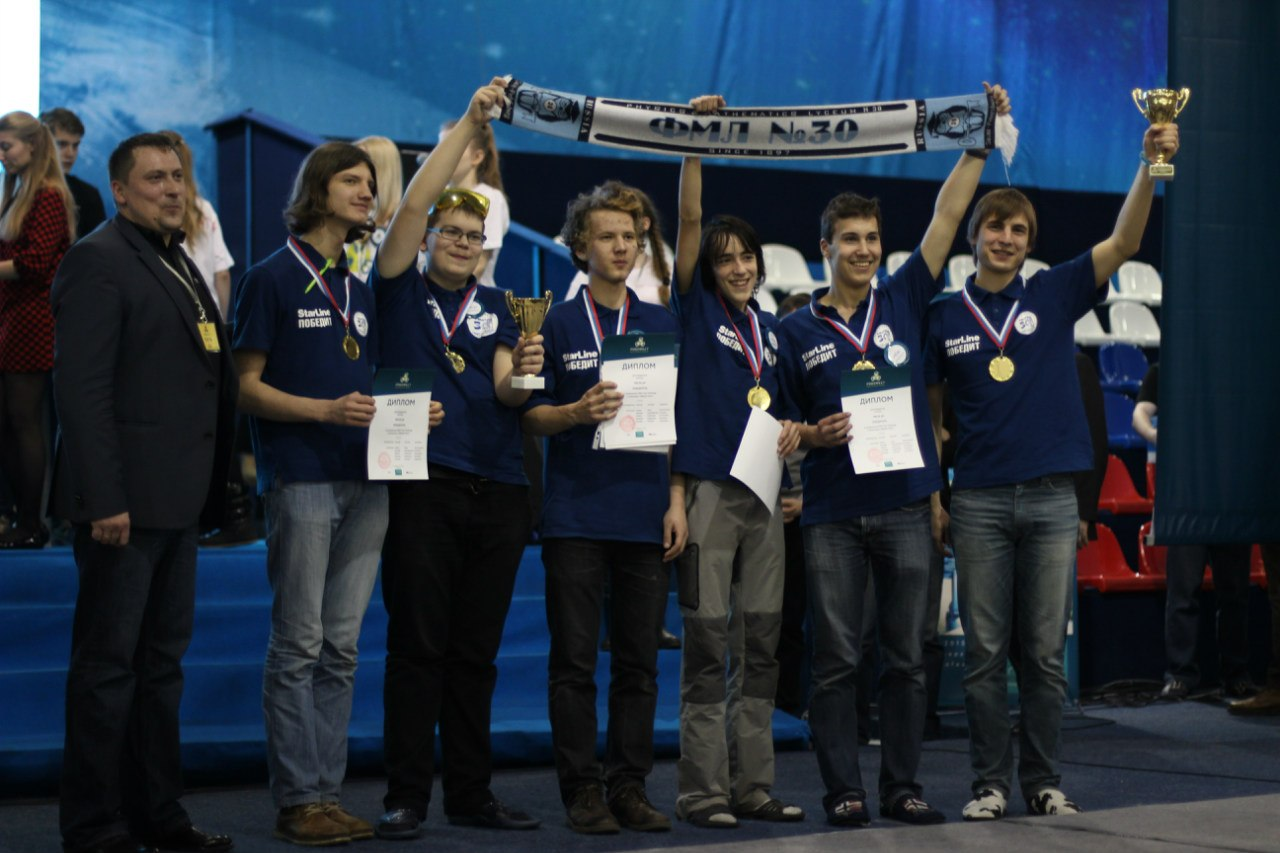
\includegraphics[scale=0.2]{key_chapters/Team/images/09}}\\
	\end{figure}[H]
\fillpage

\subsubsection{Coaches}:

\begin{figure}[H]
	
	\begin{minipage}[h]{0.47\linewidth}
		Luzin Dmitry\\
		\emph{Head of Robotics Department in Phys-Math Lyceum 30, Saint-Peterburg, Russia. Main coach of FTC team.\\}
		\emph{Information: 26 years old, in robotics 6 years, in FTC 4 years.}
	\end{minipage}
	\hfill
	\begin{minipage}{0.47\linewidth}
		\center{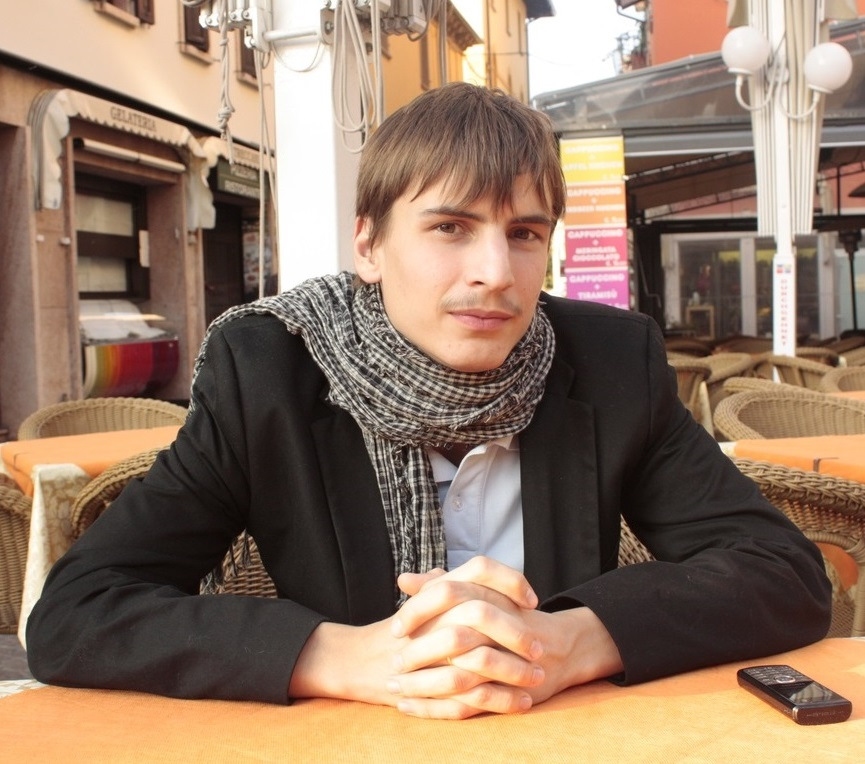
\includegraphics[scale=0.3]{key_chapters/Team/images/07}}\\
	\end{minipage}
	\vfill
	\begin{minipage}[h]{0.47\linewidth}
		\center{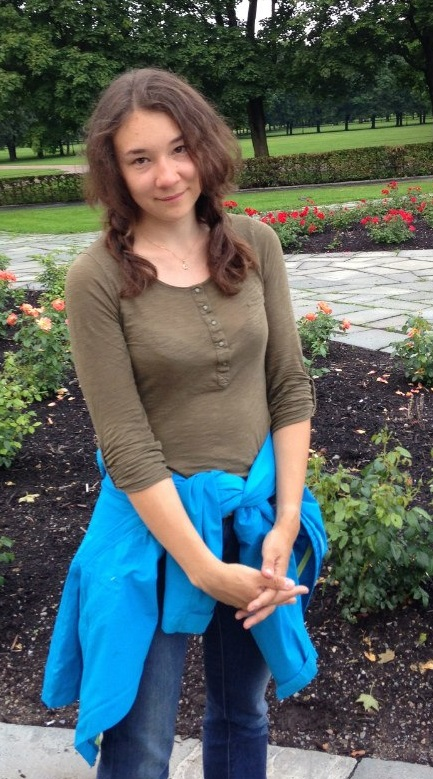
\includegraphics[scale=0.35]{key_chapters/Team/images/08}}\\
	\end{minipage}
	\hfill
	\begin{minipage}{0.47\linewidth}
		Luzina Ekaterina \\
		\emph{Professor of Robotics Department in Phys-Math Lyceum 30, Saint-Peterburg, Russia. Tutor of FTC team. \\}
		\emph{Information: 26 years old, in robotics 6 years, in FTC 4 years.}
	\end{minipage}
\end{figure}

\begin{figure}[H]
	\begin{minipage}[h]{0.47\linewidth}
		\center{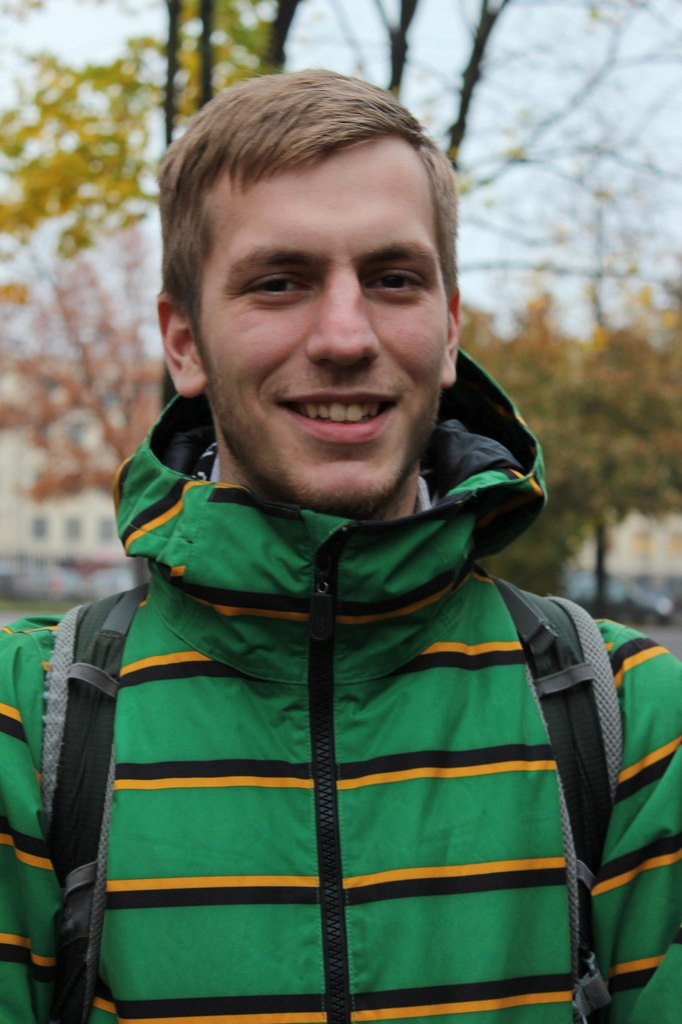
\includegraphics[scale=0.25]{key_chapters/Team/images/05}}\\
	\end{minipage}
	\hfill
	\begin{minipage}{0.47\linewidth}
		Fedotov Anton \\ 
		\emph{Professor of Robotics Department in Phys-Math Lyceum 30, Saint-Peterburg, Russia. Tutor of FTC team. \\}
		\emph{Information: 23 years old, in robotics 5 years, in FTC 4 years.}
	\end{minipage}	
	\vfill 
	\begin{minipage}{0.47\linewidth}
		Krylov Georgii \\ 
		\emph{Professor of Robotics Department in Phys-Math Lyceum 30, Saint-Peterburg, Russia. Tutor of FTC team. \\}
		\emph{Information: 18 years old, in robotics 4 years, in FTC 4 years.}
	\end{minipage}
	\hfill
	\begin{minipage}[h]{0.47\linewidth}
		\center{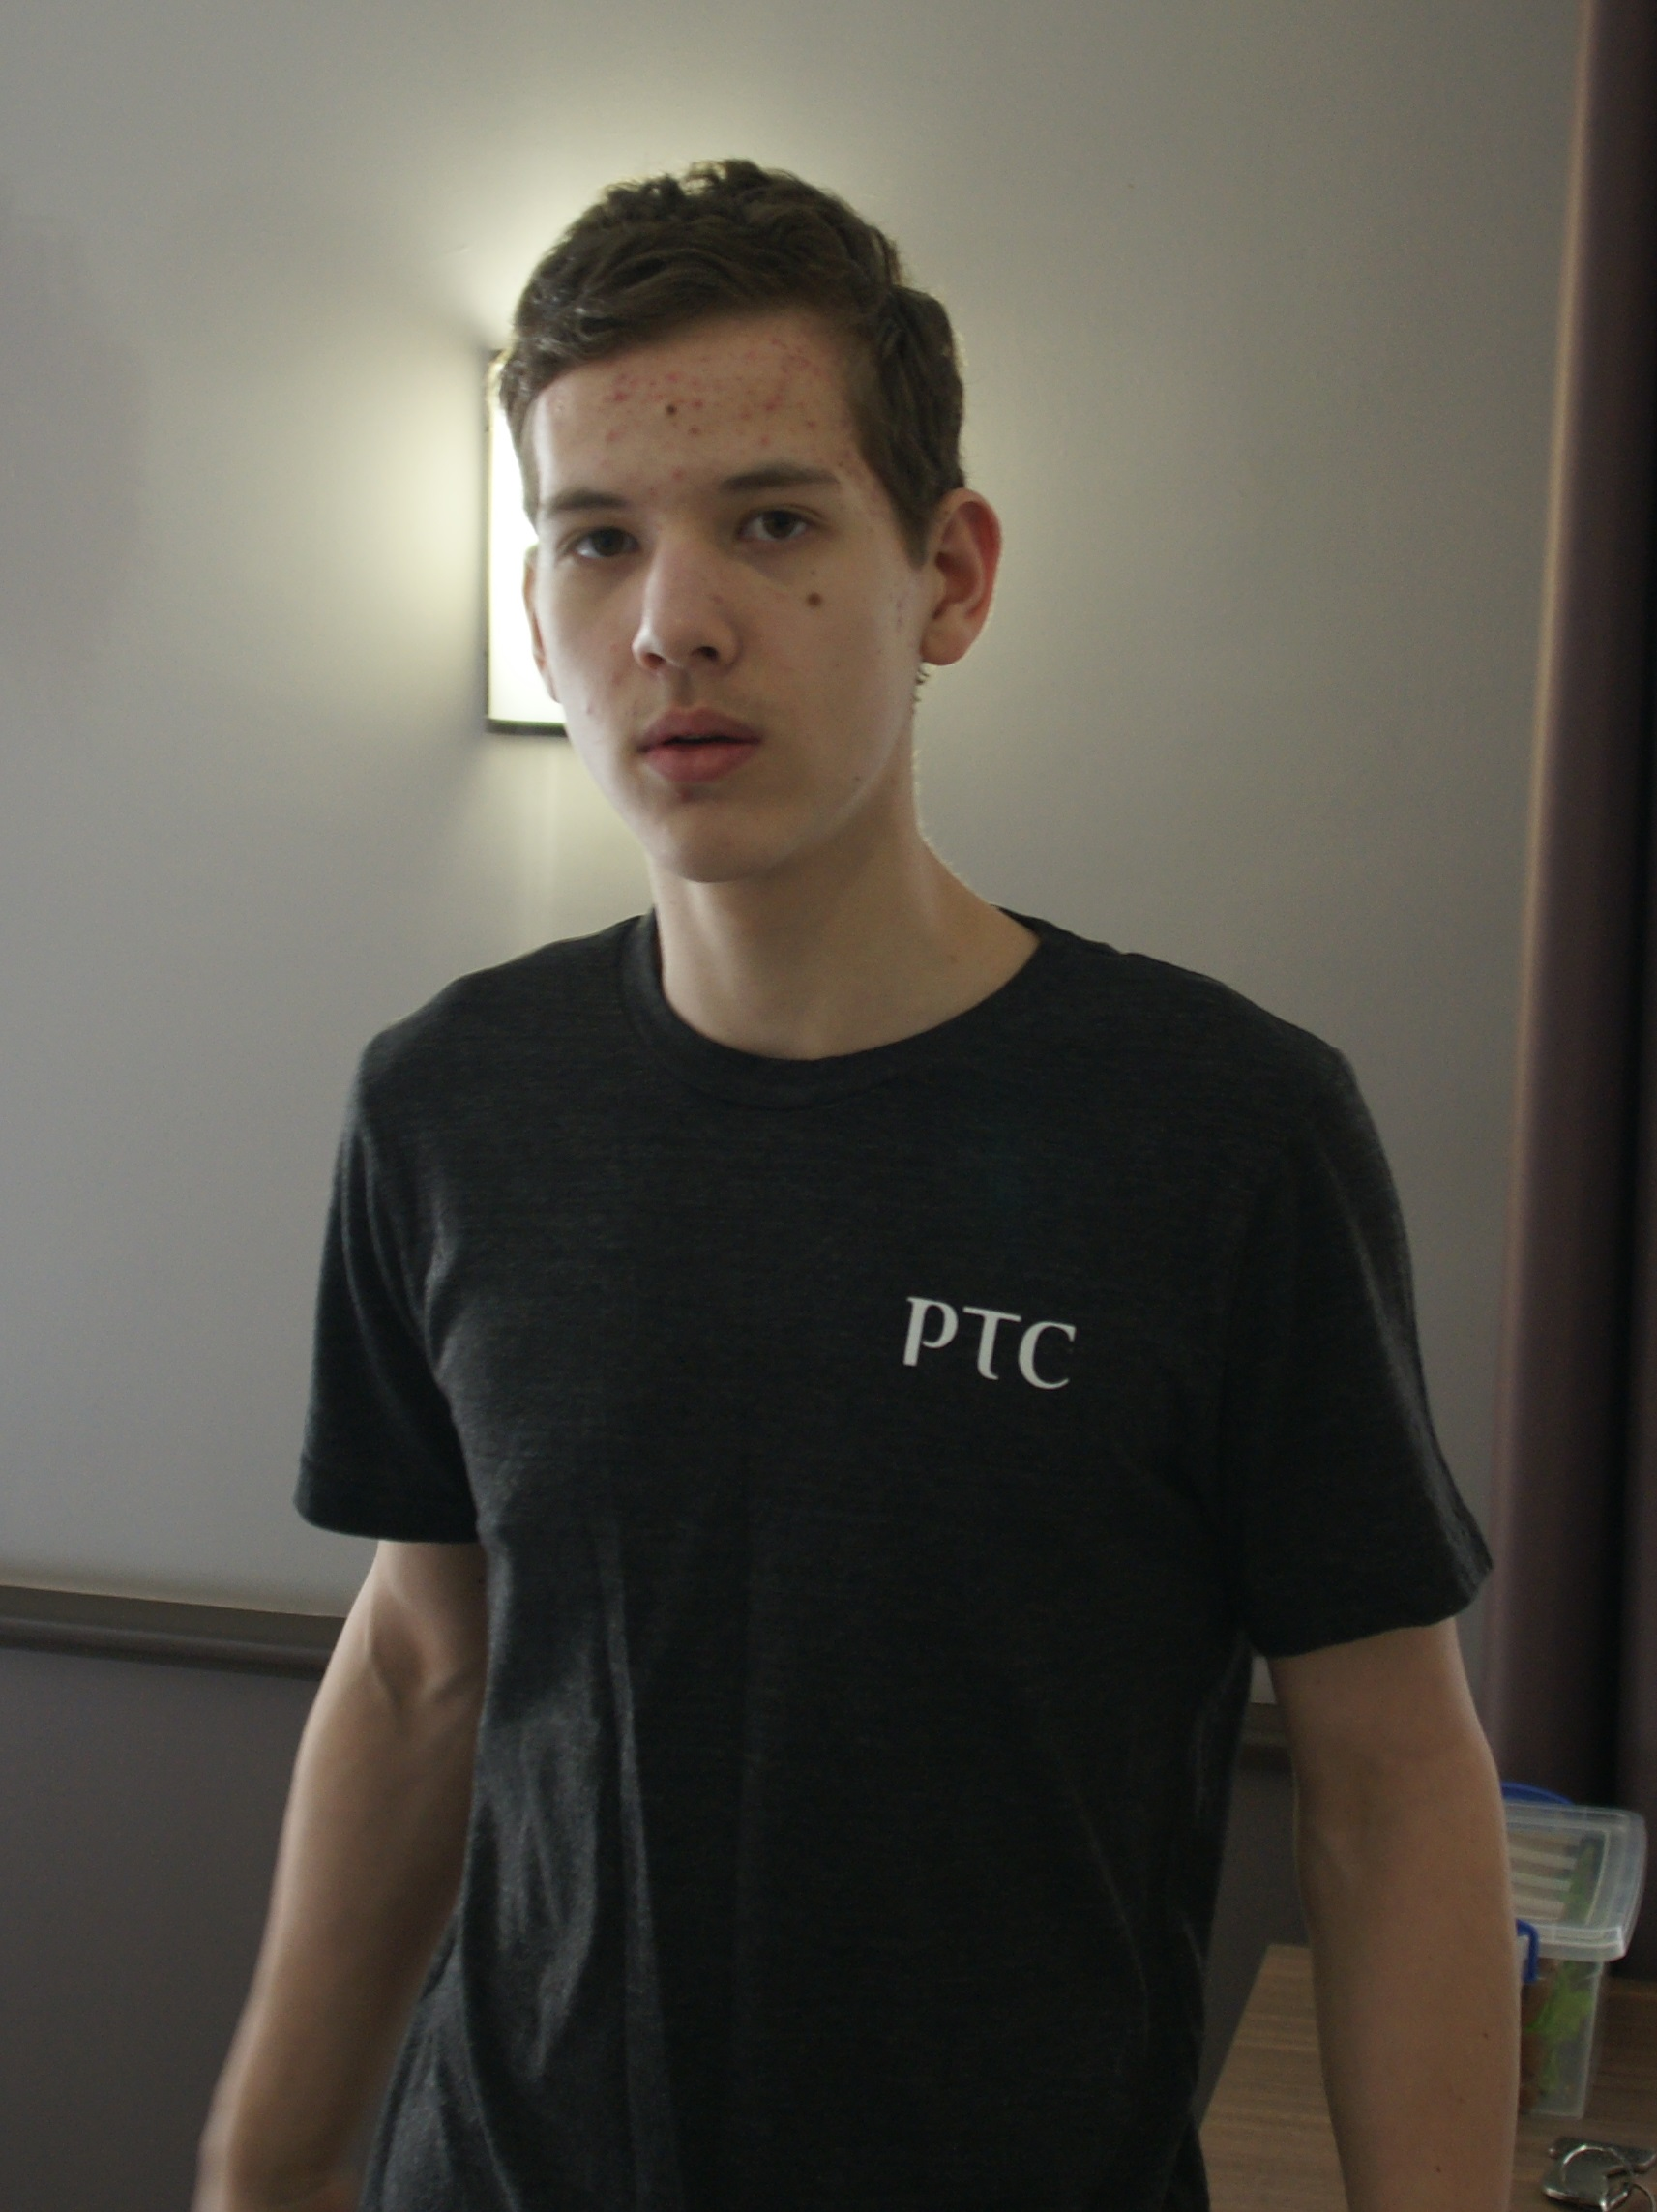
\includegraphics[scale=0.1]{key_chapters/Team/images/06}}\\
	\end{minipage}	
\end{figure}

\fillpage

\subsubsection{Team members}
\begin{figure}[H]
	\begin{minipage}[h]{0.47\linewidth}
		\center{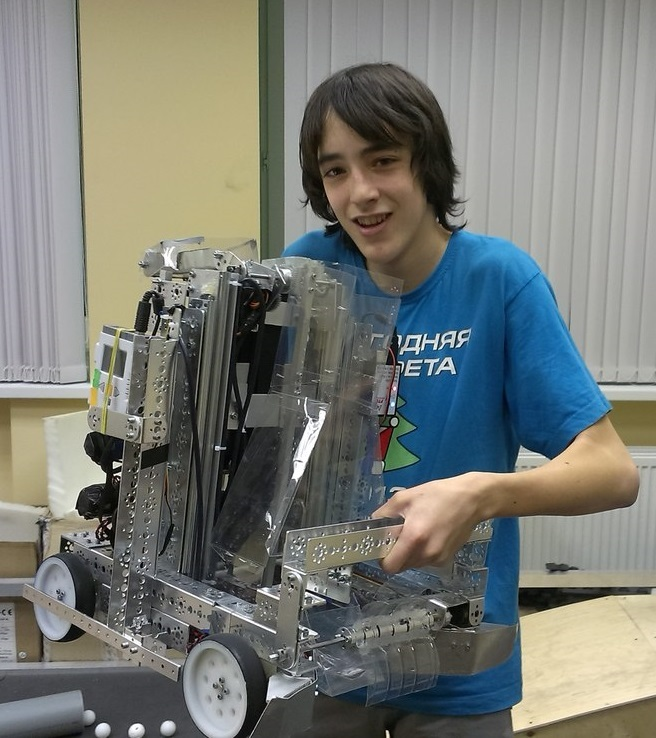
\includegraphics[scale=0.27]{key_chapters/Team/images/04}}\\		
	\end{minipage}
	\hfill
	\begin{minipage}[h]{0.47\linewidth}
		Maksimychev Evgeny\\
		\emph{Role in team: captain, operator-2, responsible for the technic of safety,  writing of engineering notebook, developer of lift and bucket for scoring elements. \\}
		\emph{Information: 16 years old, in robotics 3 years, in FTC 2 year. \\}
		\emph{Why I chose FTC: "This is an interesting project that allows to implement some innovative solutions. In addition to the skills of designing robots, we also obtain the skills of the technical documentation and communication with colleagues which makes this competition close to real engineering problems."}	
	\end{minipage}
\end{figure}
	\vfill 
	\begin{figure}[H]
	\begin{minipage}[h]{0.47\linewidth}
		Timur Babadzhanov\\
		\emph{Role in team: operator-1,  developer mechanism for scoring autonomous climbers\\ }
		\emph{Information: 15 years old, in robotics 2 years, in FTC 1 years. \\ } 
		\emph{Why I chose FTC:" It was recommended for me. Also I heared about previous seasons of FTC and decided that it will be interesting for me. Also I wanted to learn working with TETRIX that can be useful for my projects."}					
	\end{minipage}
	\hfill
	\begin{minipage}[h]{0.47\linewidth}
		\center{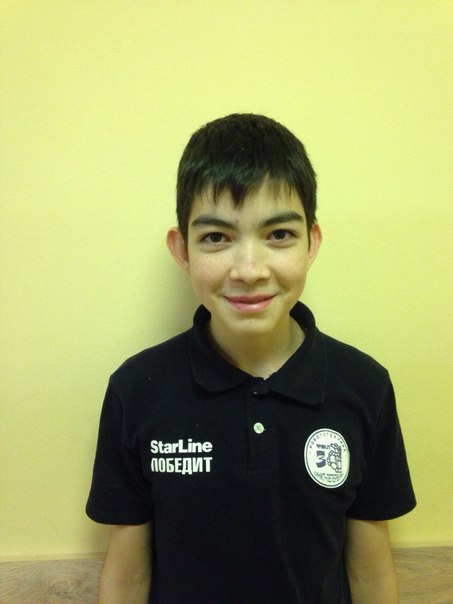
\includegraphics[scale=0.4]{key_chapters/Team/images/01}}\\
	\end{minipage}
\end{figure}
\hfill

\begin{figure}[H]	
	\begin{minipage}{0.47\linewidth}
		\center{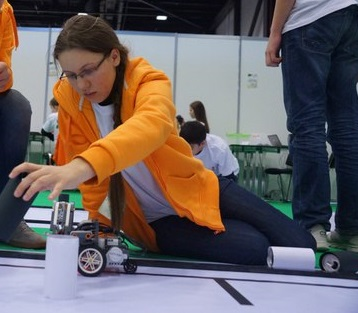
\includegraphics[scale=0.7]{key_chapters/Team/images/11}}					
	\end{minipage}
	\hfill
	\begin{minipage}{0.47\linewidth}
		Victoria Loseva\\
		\emph{Role in team: developer of wheel base, programmer\\ }
		\emph{Information: 17 years old, in robotics 2 years, in FTC 1 years. \\} 
		\emph{Why I chose FTC:"I enjoy working on new and unique projects, and FTC is a great way for me to do exactly that: solving the challenging problem of building and designing a robot from scratch, as a team, is all FTC is about!"}			
	\end{minipage}
\end{figure}
\fillpage


